%% SW design: klassebeskrivelse SPI API

\begin{figure}[htbp] \centering
{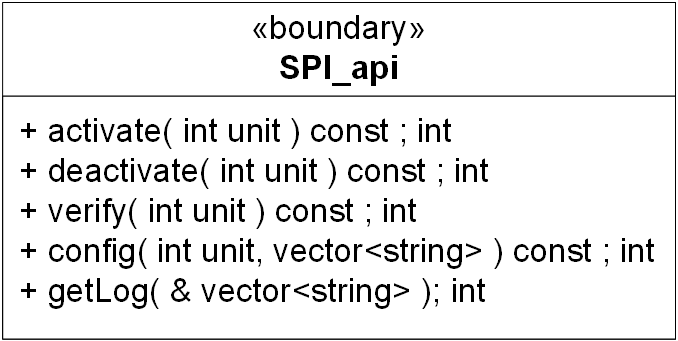
\includegraphics[scale=1.5]{filer/design/Klassediagrammer/SPI_API}}
\caption{klassediagram SPI API}
\label{fig:SPI API klassediagram}
\end{figure} 

{\centering
\textbf{SPI\_api}\par
}
\textbf{Ansvar:} At være et lag imellem \textit{applications}-laget og \textit{device driver}-laget ifm. SPI kommunikation. \

\verb+int activate( int unit ) const +\\
\textbf{Parametre:} Modtager en integer på Enhed som skal aktiveres. \\
\textbf{Returværdi:} 0 ved succes ellers negativ i overenstemmelse med fejl-listen. \\
\textbf{Beskrivelse:} Metoden skal aktivere Enheden \verb+unit+ over SPI netværket.\\

\verb+int deactivate( int unit ) const+ \\
\textbf{Parametre:}  Modtager en integer på følgende Enhed som skal deaktiveres.\\
\textbf{Returværdi}: 0 ved succes ellers negativ i overenstemmelse med fejl-listen. \\
\textbf{Beskrivelse:} Metoden skal deaktivere Enheden \verb+unit+ over SPI netværket.\\

\verb+int verify( int unit ) const+ \\
\textbf{Parametre:}  Modtager en integer på følgende Enhed som skal verificeres.\\
\textbf{Returværdi:} 0 ved succes ellers negativ i overenstemmelse med fejl-listen.   \\
\textbf{Beskrivelse:} Metoden skal verificere om Enheden \verb+unit+ er tilkoblet SPI netværket.\\

\verb+int config( int unit, float temp, float humi ) const +\\
\textbf{Parametre:} Modtager en integer på følgende Enhed som skal konfigureres. Derudover modtager den to floats med parametrene som skal skrives til Enhed. \\
\textbf{Returværdi:}  0 ved succes ellers negativ i overenstemmelse med fejl-listen.   \\
\textbf{Beskrivelse:} Metoden skal sende konfigurations-parametrene i \verb+float+ til Enheden \verb+unit+ over SPI netværket.\\

\verb+int getLog( & vector<string> , int * units, int size )+ \\
\textbf{Parametre:}  Modtager en referance til en vector af typen string som loggen skal gemmes i. Pointer til array af Enheder som skal logges samt int med antallet af Enheder i arrayet. \\
\textbf{Returværdi:}  0 ved succes ellers negativ i overenstemmelse med fejl-listen.   \\
\textbf{Beskrivelse:} Metoden skal hente log fra Enheder i arrayet \verb+units+ på SPI netværket og gemme dem i \verb+vector+ i henhold til dataprotokollen. \\
